\documentclass[
	letterpaper, % Paper size, specify a4paper (A4) or letterpaper (US letter)
	10pt, % Default font size, specify 10pt, 11pt or 12pt
]{CSUniSchoolLabReport}

%----------------------------------------------------------------------------------------
%	REPORT INFORMATION
%----------------------------------------------------------------------------------------

\title{Introduction to Adders \\ Embedded Design: Enabling Robotics \\ EECE2160} % Report title

\author{Michael \textsc{Brodskiy}\\ \small \href{mailto:Brodskiy.M@Northeastern.edu}{Brodskiy.M@Northeastern.edu}}

\date{February 4, 2023} % Date of the report

%----------------------------------------------------------------------------------------


\begin{document}

\maketitle % Insert the title, author and date using the information specified above

\begin{center}
	\begin{tabular}{l r}
		Date Performed: & January 26, 2023 \\ % Date the experiment was performed
        Partner: & Dylan \textsc{Powers} \\ % Partner names
		Instructor: & Professor \textsc{Shazli} % Instructor/supervisor
	\end{tabular}
\end{center}

\newpage

\begin{abstract}

  First and foremost, this laboratory experiment introduces the Quartus utility as it pertains to interacting with the embedded design of circuit boards. Following a brief introduction, a half-adder was constructing. By utilizing two of the half-adder constructions, a full-adder was assembled. This full-adder was used to construct higher bit adders — more specifically 8 bits, in the case of this lab. The following document outlines the progression of the lab work.

\end{abstract}

\begin{flushleft}

  \textsc{Keywords:} \underline{Quartus}, \underline{circuit board}, \underline{half-adder}, \underline{full-adder}, \underline{adder}

\end{flushleft}

\newpage

\section{Introduction}

\hspace{.5 in}    This laboratory experiment allowed for a quick introduction into the world of embedded design by guiding the user through a series of embedded design tools, concepts, and critical thinking. This includes the orientation of the user to the Quartus Prime Lite software, used to construct, package, and embed logic gate designs. The knowledge of truth tables was built upon when it was necessary to construct adders.\newline

\hspace{.5 in}    The first adder to be constructed was the half-adder. Half-adders add together two single bits to produce a sum value and a carry value. A value of 1 for the sum indicates that one of the bits is zero and the other is 1, while a value of 1 for carry indicates that both bits are equal to 1. Thus, carry would mean that a 1 is passed to the next bit, which is useful for constructing larger adders. \newline

\hspace{.5 in}    As such, the next adder to be constructed was a full-adder, which consists of two half-adders. The full-adder also adds two single bits, but it is useful in that it consists of three inputs, instead of two as with the half-adder. This can be used to construct larger bit adders, as the additional input can be used to add in a carry from the previous bits. \newline

\hspace{.5 in}    Consequently, it is logical that the next adder to be constructed was a multi-bit adder, in this case consisting of 8 bits. This consists of 8 full-adders (or 16 half-adders), and is able to sum two 8-bit numbers, as well as tracking for overflow. Because the board only contains 10 switches, the first number is fully variable, while the second number's first 6 bits were set to ones. In this manner, the lab taught the importance of truth table construction, as well as the significance of adders.

\section{Discussion \& Analysis} 

\hspace{.5 in} Adders are used to add any two $n$-bit numbers. A half-adder, the first design to be constructed (as shown in Figure \ref{fig:1}), was used to add two single bits, and output a sum and carry term. The schematic was then functionally simulated and packed onto the De1-SoC board used for the lab. As shown in Figure \ref{fig:2}, both switches (bits) are turned on (set to 1). This results in a sum value of 0 (as shown by the light above the first switch), and a carry value of 1 (as shown by the light above the second switch. This makes sense, as the addition of two one bits would generate a carry over to the next bit. \newline

  \hspace{.5 in} This was then used for the full-adder. The design of the full-adder can be seen in Figure \ref{fig:3}. The full-adder, as stated above, consists of two half-adders, and has one more input than a half-adder, allowing for the easy construction of multi-bit adders. To confirm the digital logic circuit was correctly constructed, extensive functional simulations were performed to ensure valid results. The test results are shown in Figure \ref{fig:4}. Finally, Figures \ref{fig:5}, \ref{fig:6}, and \ref{fig:7} show different configurations of full adder inputs. Three cases are shown; the first has a single 1 bit passed in, resulting in a sum of one and no carry, which makes sense logical, as there would be nothing to carry when a 1 is added to zero bits. Next, two 1 bits are added, which results in a carry, but no sum, as the whole value would move up a significant bit. Finally, three 1 bit values are added, which results in both a sum and carry of 1, as there is both something to carry and something left behind. \newline

  \hspace{.5 in} The final and most painstaking part of the lab was to construct an eight bit adder from scratch. This means it should add two eight bit numbers. Due to the lack of switches on the De1-SoC board, the six most significant bits of the second number were set to ones. The digital circuit was constructed in two ways: one in which the two eight bit numbers are fully variable, and one where the second number only varies in its two least significant bits. These designs are shown in Figures \ref{fig:8} and \ref{fig:9}, respectively. To confirm the validity of the fully-variable eight bit adder, extensive tests were run, as well as an abridged version of tests for easier analysis, as shown in Figures \ref{fig:10} and \ref{fig:11}. The shortened tests demonstrate two cases: one with overflow and one without. Figures \ref{fig:12} and \ref{fig:13} show the 8-bit adder in overflow and in a normal state, respectively. The overflow is detected if a carry bit is released from the addition of the leading bits of the two numbers. In such a case, the ninth light would turn on to indicate there was a bit overflow. Because the second number six leading ones, a one in any of the first six bits of the first number would lead to overflow, as shown in Figure \ref{fig:12}. This problem does not occur in Figure \ref{fig:13} because only the first two are triggered. \newline

  \hspace{.5 in} Because no measurements were taken during this lab, there are no major sources of error.

  \section{Conclusion}

  \hspace{.5 in} Overall, the lab provided a well-coordinated introduction to embedded design. By slowly demonstrating how to convert truth tables to digital logic circuits, and smaller circuits into larger, more integrated circuits, it was easy to learn the software and physical processes involved. As such, the lab provides an adequate introduction into embedded design.

  \newpage

\section{Appendix}

\begin{figure}[h!]
  \centering
  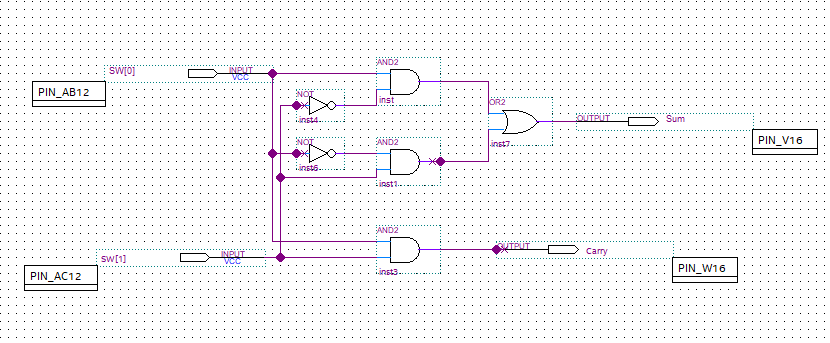
\includegraphics[width=.9\textwidth]{Figures/HalfAddDesign.png}
  \caption{The Half-Adder Schematic Design}
  \label{fig:1}
\end{figure}

\begin{figure}[h!]
  \centering
  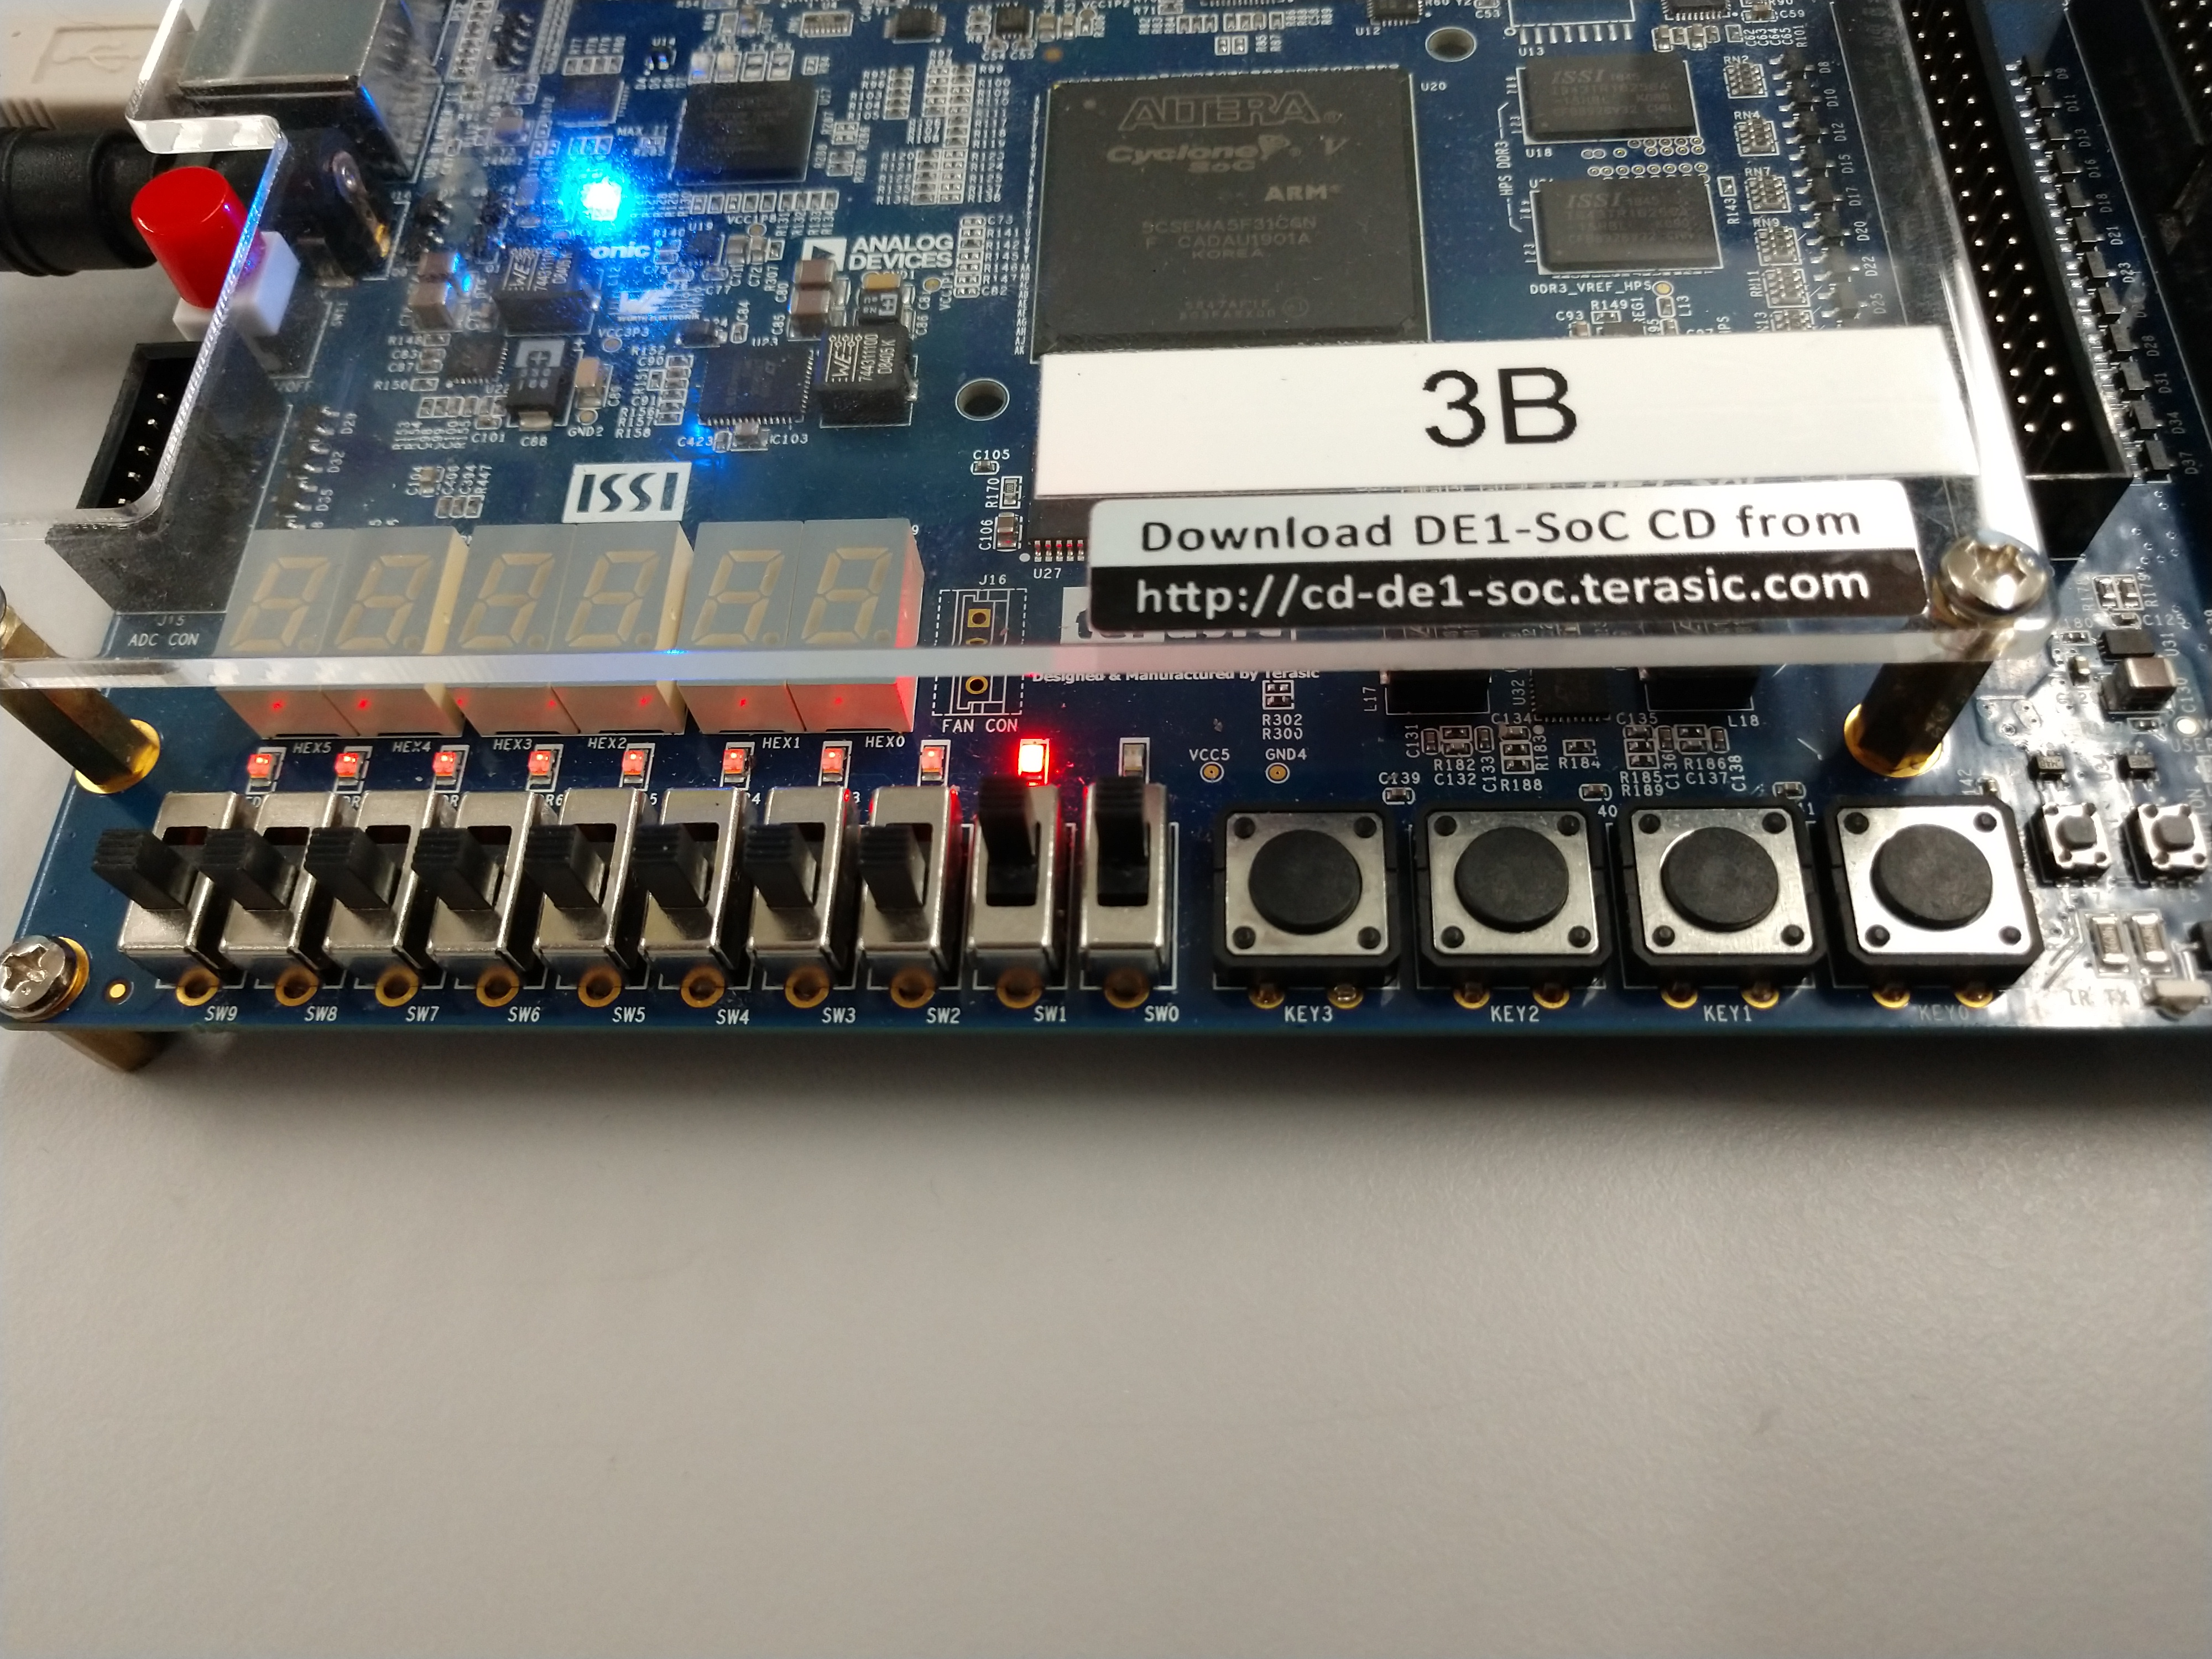
\includegraphics[width=.9\textwidth]{Figures/HalfAdder.jpg}
  \caption{Half-Adder Test with Both Bits (Switches) Set to 1}
  \label{fig:2}
\end{figure}

\begin{figure}[h!]
  \centering
  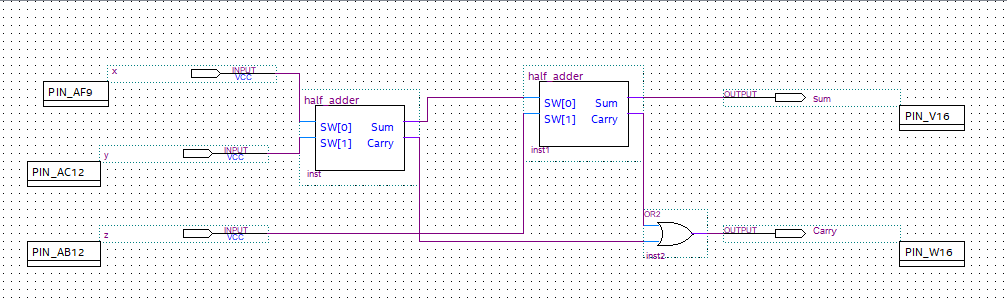
\includegraphics[width=.9\textwidth]{Figures/FullAdderDesign.png}
  \caption{The Full-Adder Schematic Design}
  \label{fig:3}
\end{figure}

\begin{figure}[h!]
  \centering
  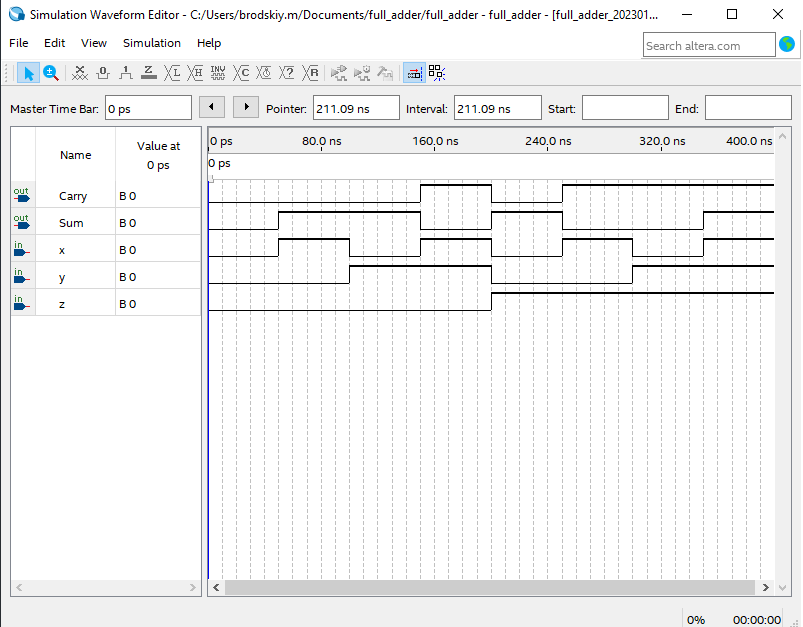
\includegraphics[width=.9\textwidth]{Figures/FullAddSim.png}
  \caption{The Full-Adder Simulation Results}
  \label{fig:4}
\end{figure}

\begin{figure}[h!]
  \centering
  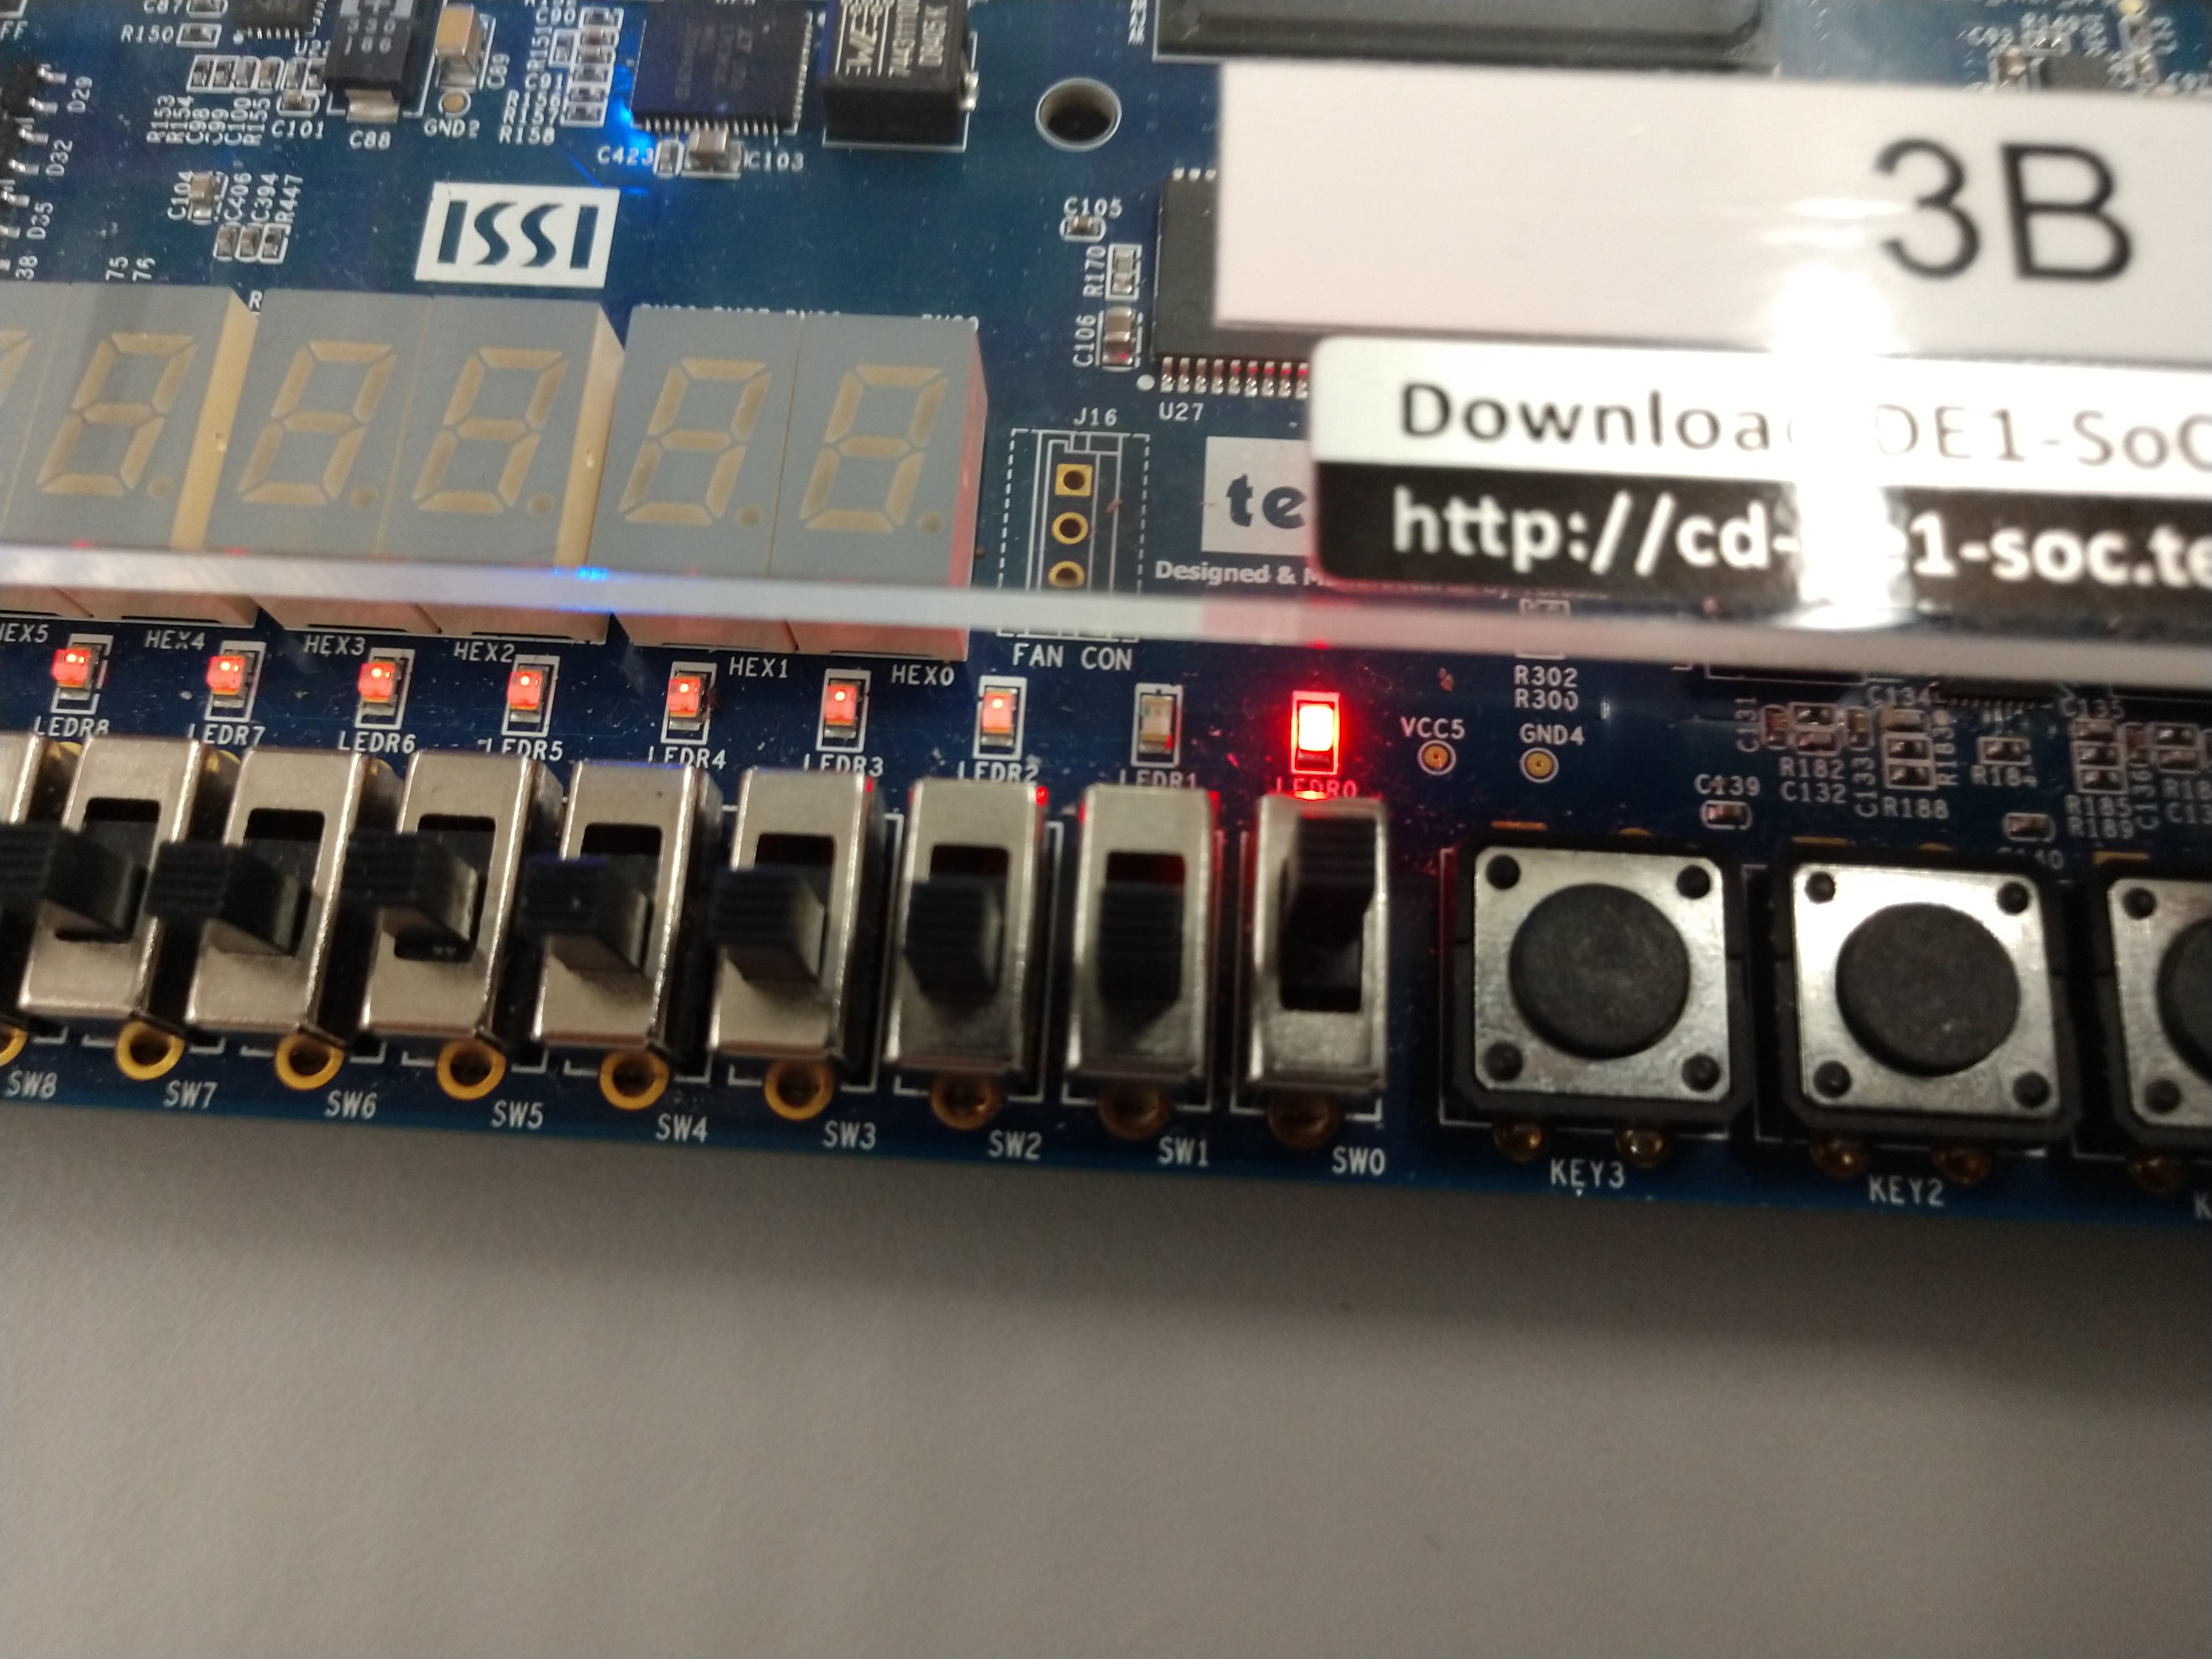
\includegraphics[width=.9\textwidth]{Figures/FullAdd1.jpg}
  \caption{Full-Adder with A Single 1 Bit (Carry is 0, Sum is 1)}
  \label{fig:5}
\end{figure}

\begin{figure}[h!]
  \centering
  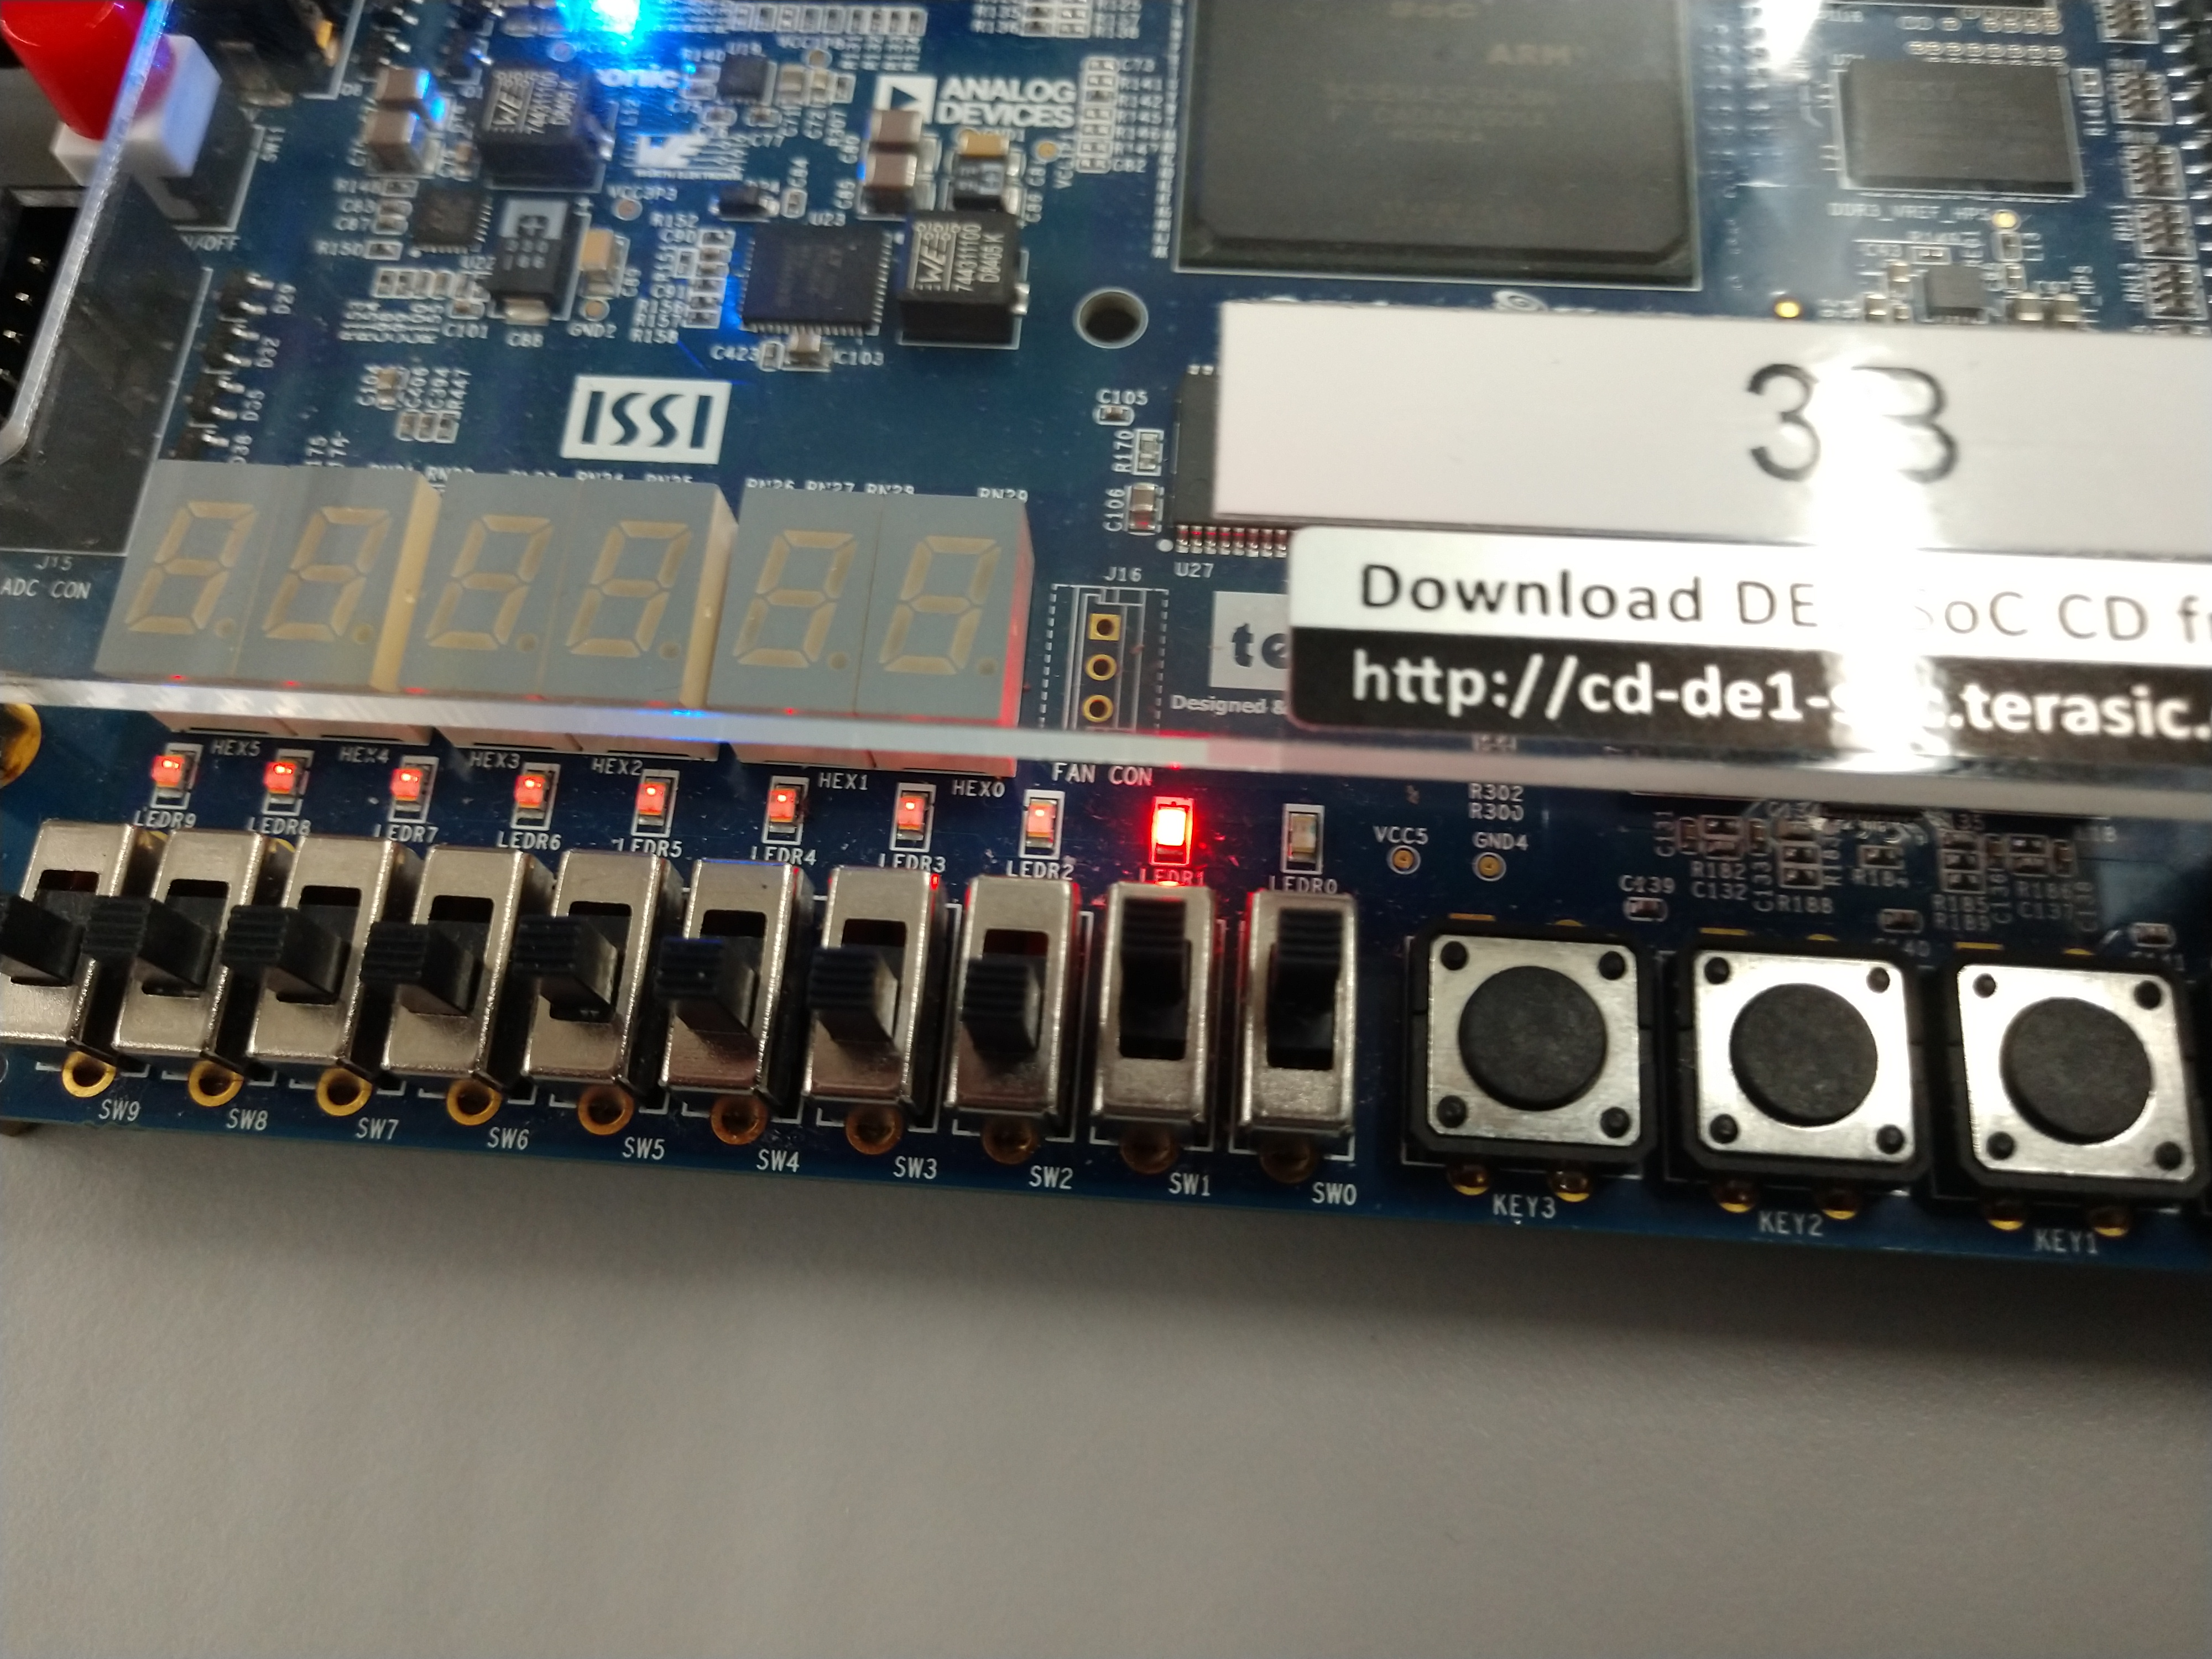
\includegraphics[width=.9\textwidth]{Figures/FullAdd2.jpg}
  \caption{Full-Adder with Two 1 Bits (Carry is 1, Sum is 0)}
  \label{fig:6}
\end{figure}

\begin{figure}[h!]
  \centering
  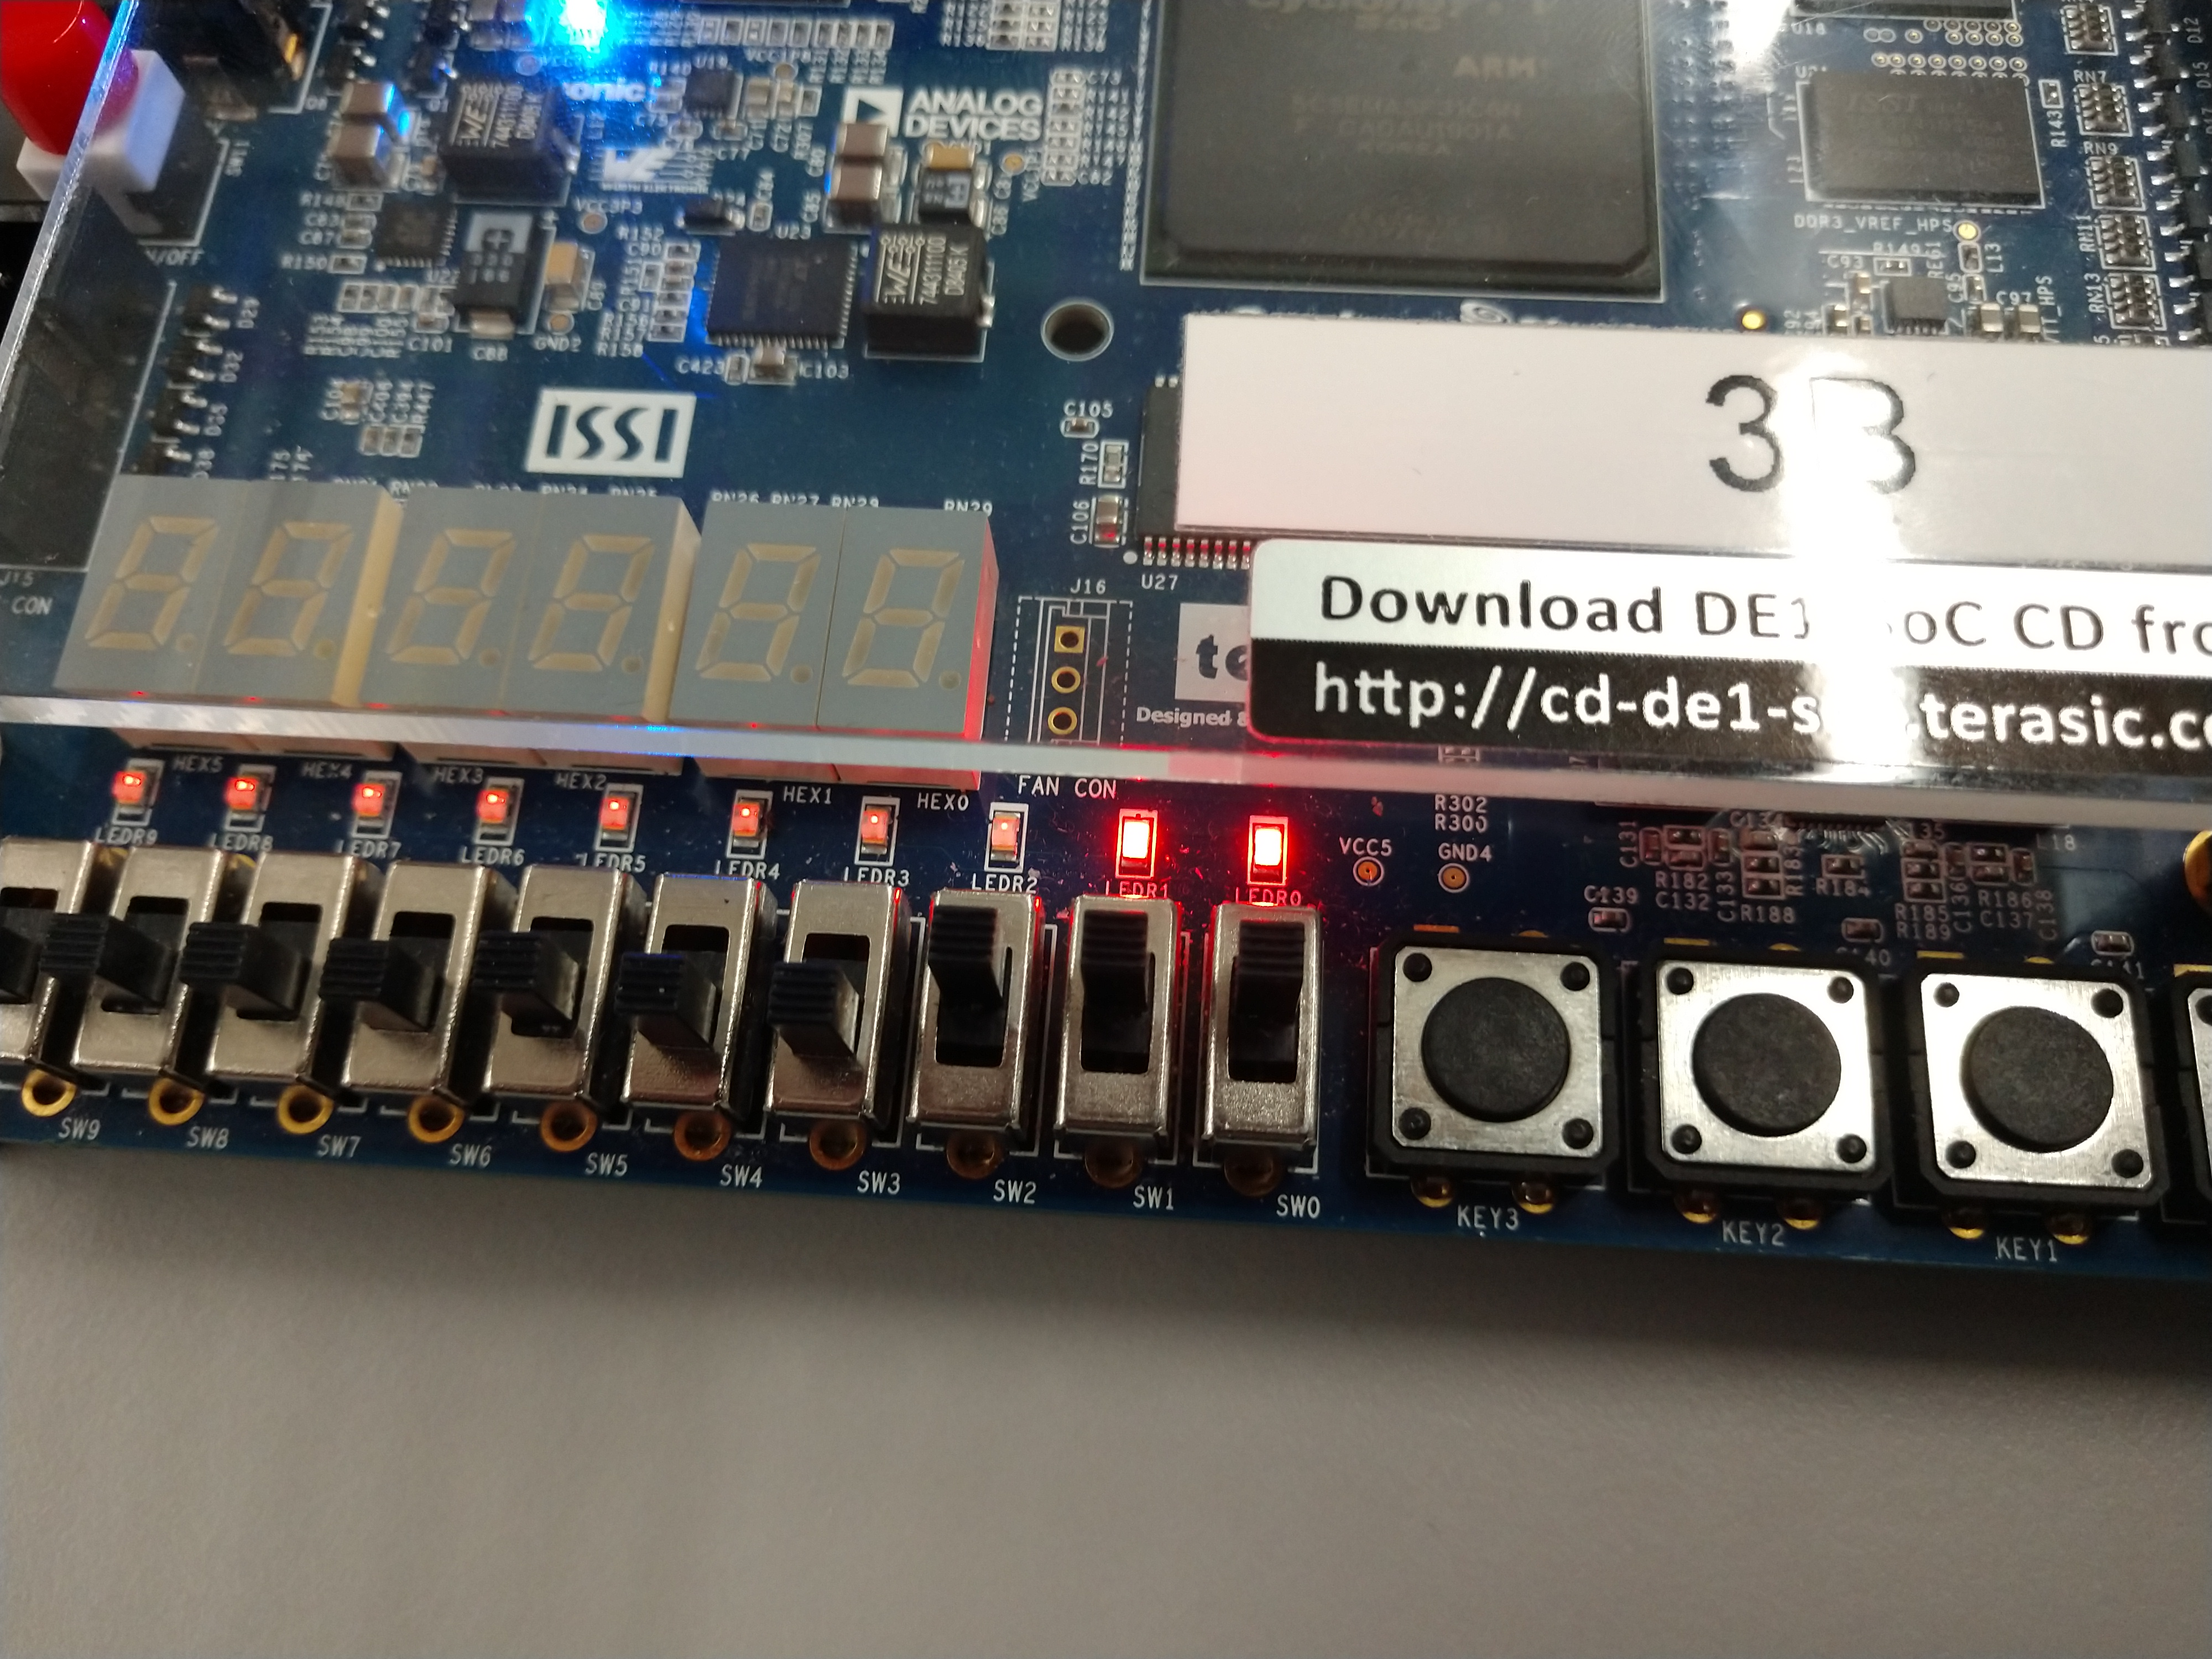
\includegraphics[width=.9\textwidth]{Figures/FullAdd3.jpg}
  \caption{Full-Adder with Three 1 Bits (Carry is 1, Sum is 1)}
  \label{fig:7}
\end{figure}

\begin{figure}[h!]
  \centering
  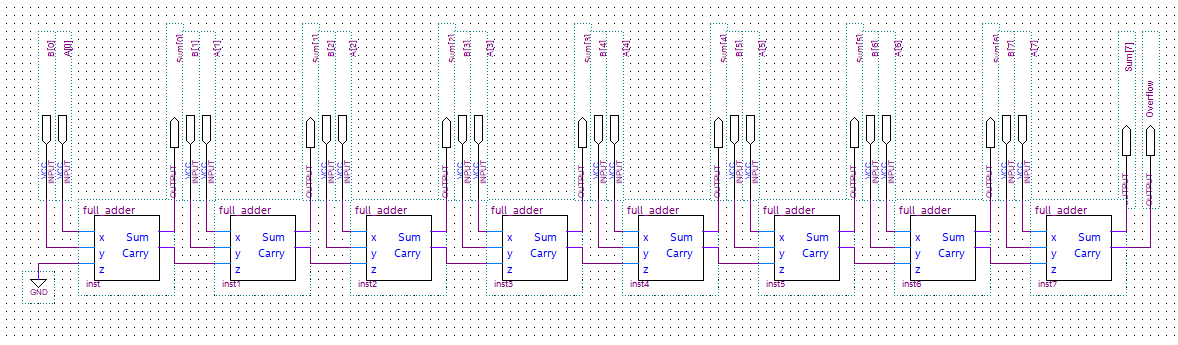
\includegraphics[width=.9\textwidth]{Figures/8BAdderFull.png}
  \caption{A Fully Variable 8-Bit Adder Schematic Design}
  \label{fig:8}
\end{figure}

\begin{figure}[h!]
  \centering
  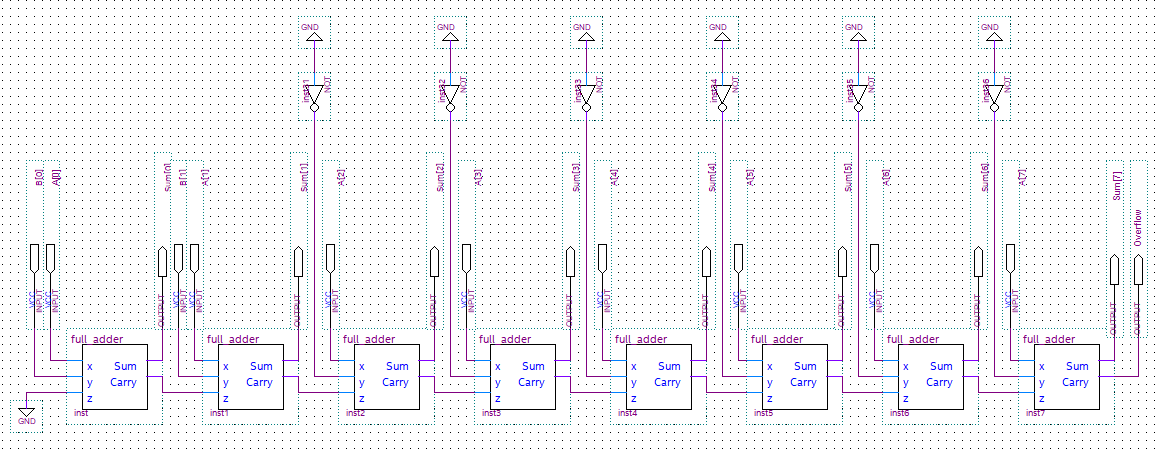
\includegraphics[width=.9\textwidth]{Figures/8BAdderForBoard.png}
  \caption{The 8-Bit Adder Design Implemented on the De1-SoC Board}
  \label{fig:9}
\end{figure}

\begin{figure}[h!]
  \centering
  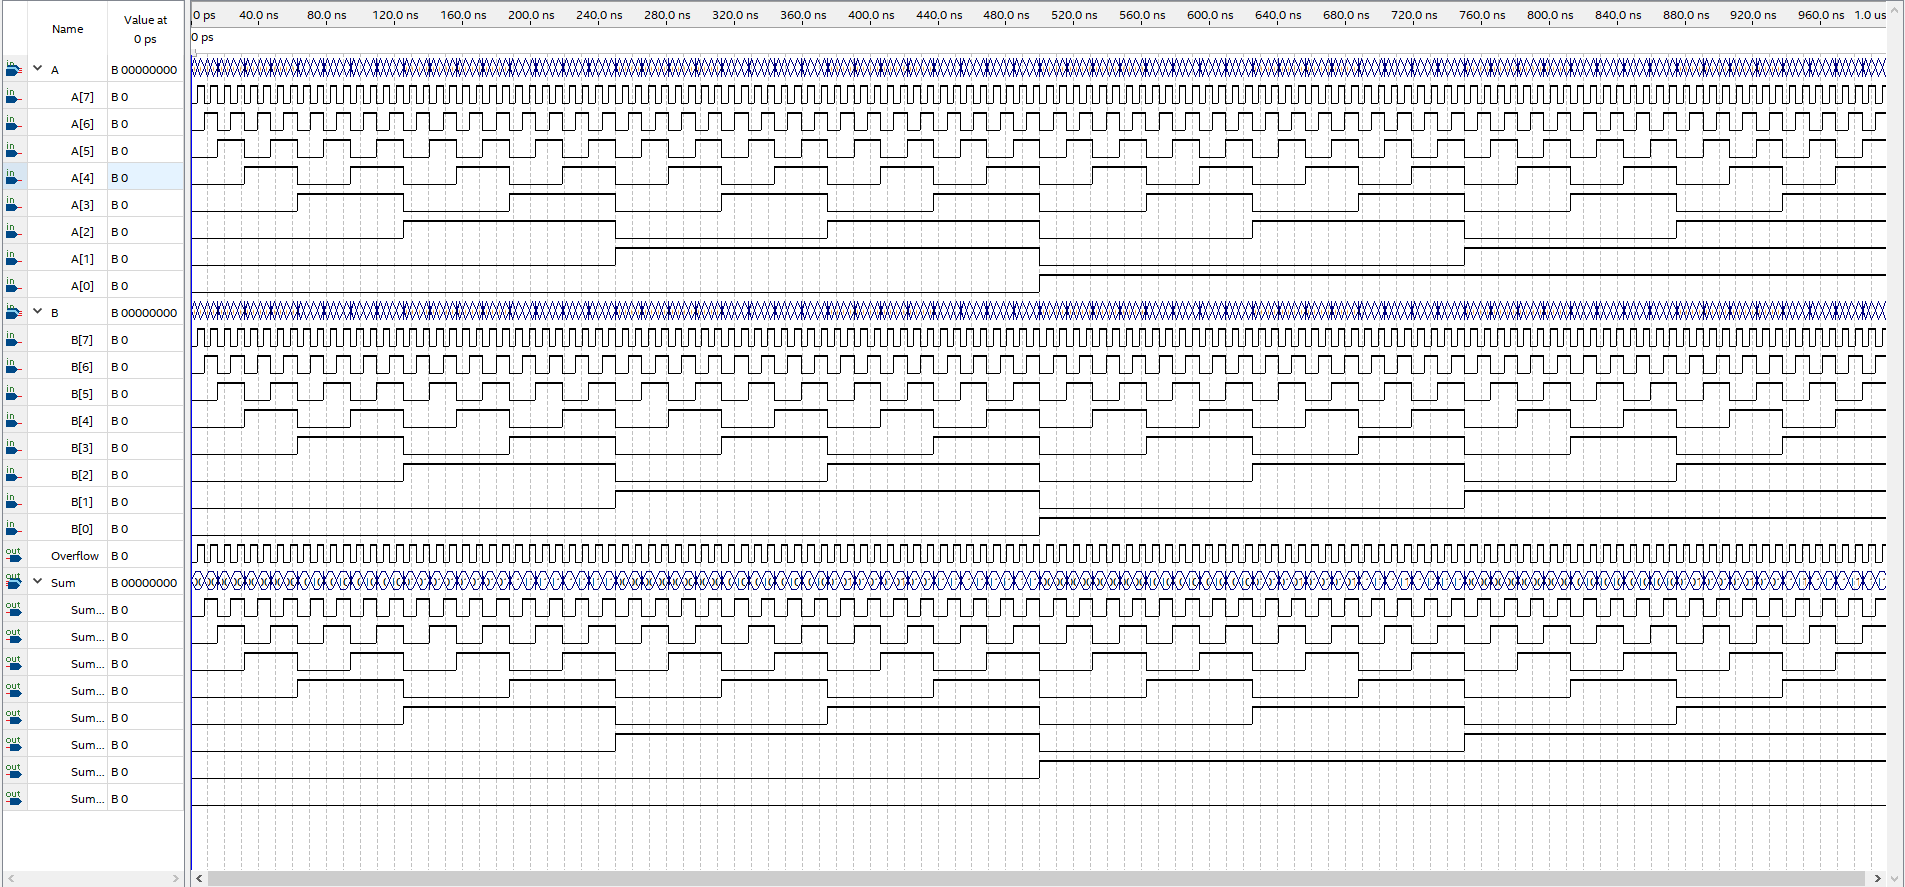
\includegraphics[width=.9\textwidth]{Figures/8BSimFull.png}
  \caption{Full 8-Bit Adder Tests}
  \label{fig:10}
\end{figure}

\begin{figure}[h!]
  \centering
  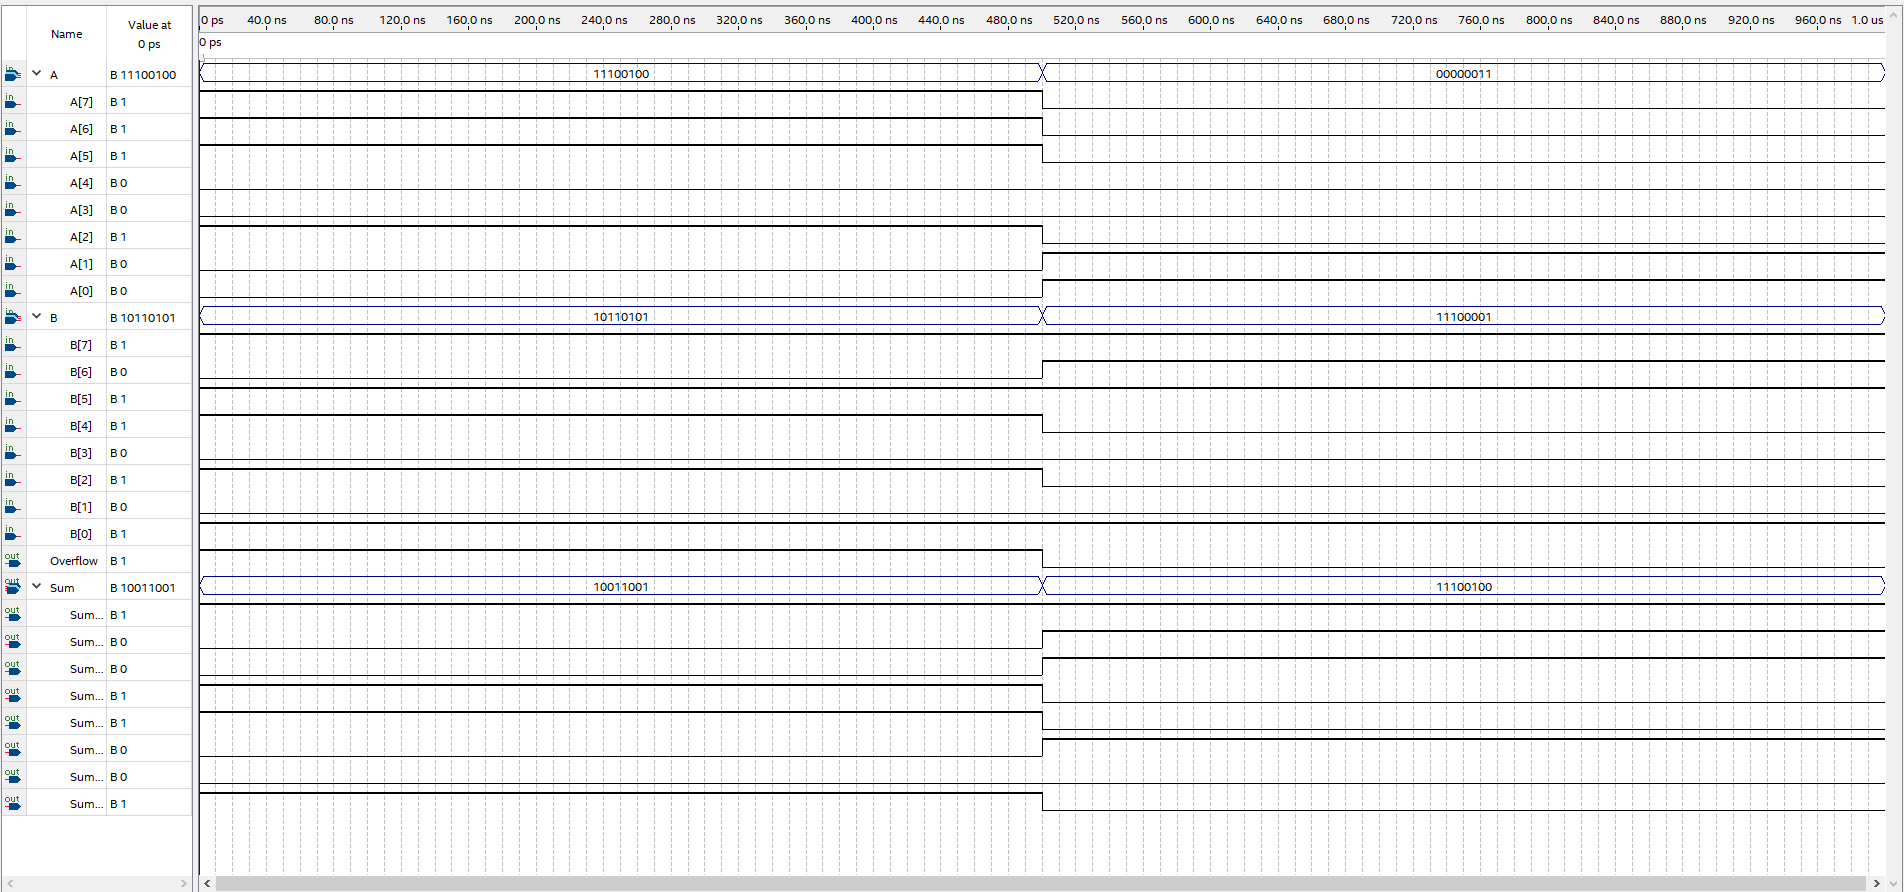
\includegraphics[width=.9\textwidth]{Figures/8BSimShort.png}
  \caption{Shortened 8-Bit Adder Tests}
  \label{fig:11}
\end{figure}

\begin{figure}[h!]
  \centering
  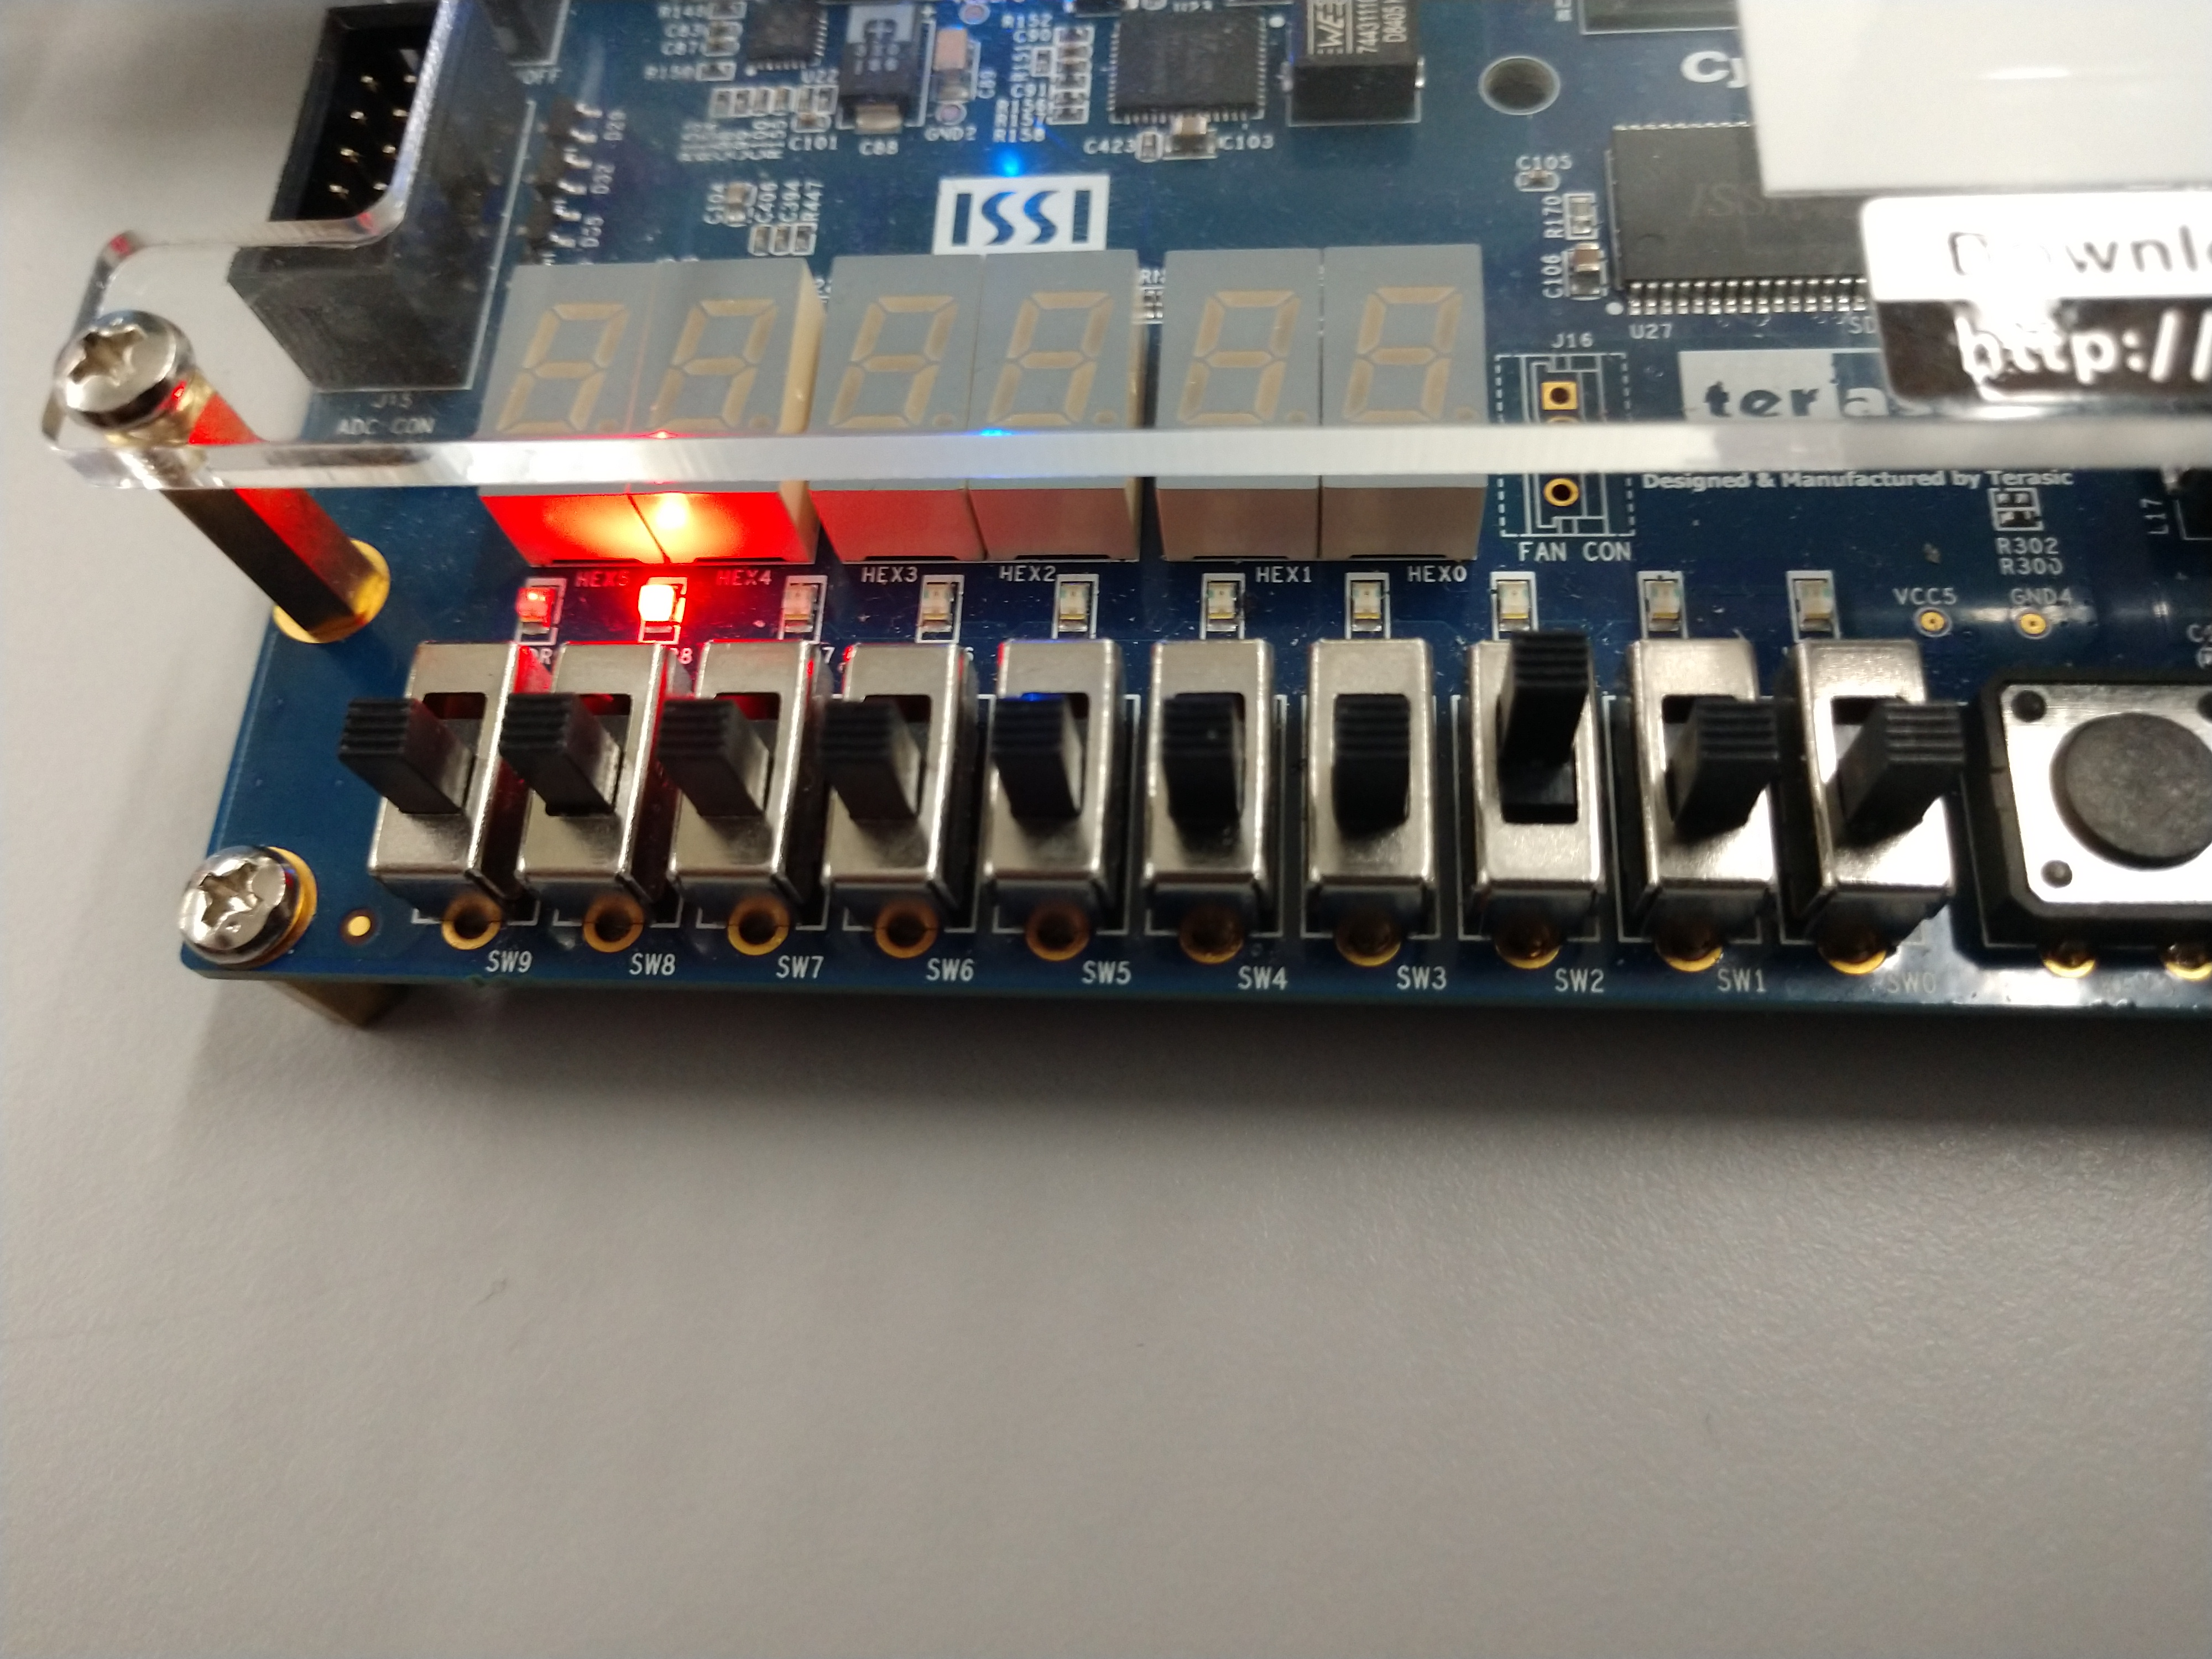
\includegraphics[width=.9\textwidth]{Figures/8BOverflow.jpg}
  \caption{8-Bit Adder in Overflow}
  \label{fig:12}
\end{figure}

\begin{figure}[h!]
  \centering
  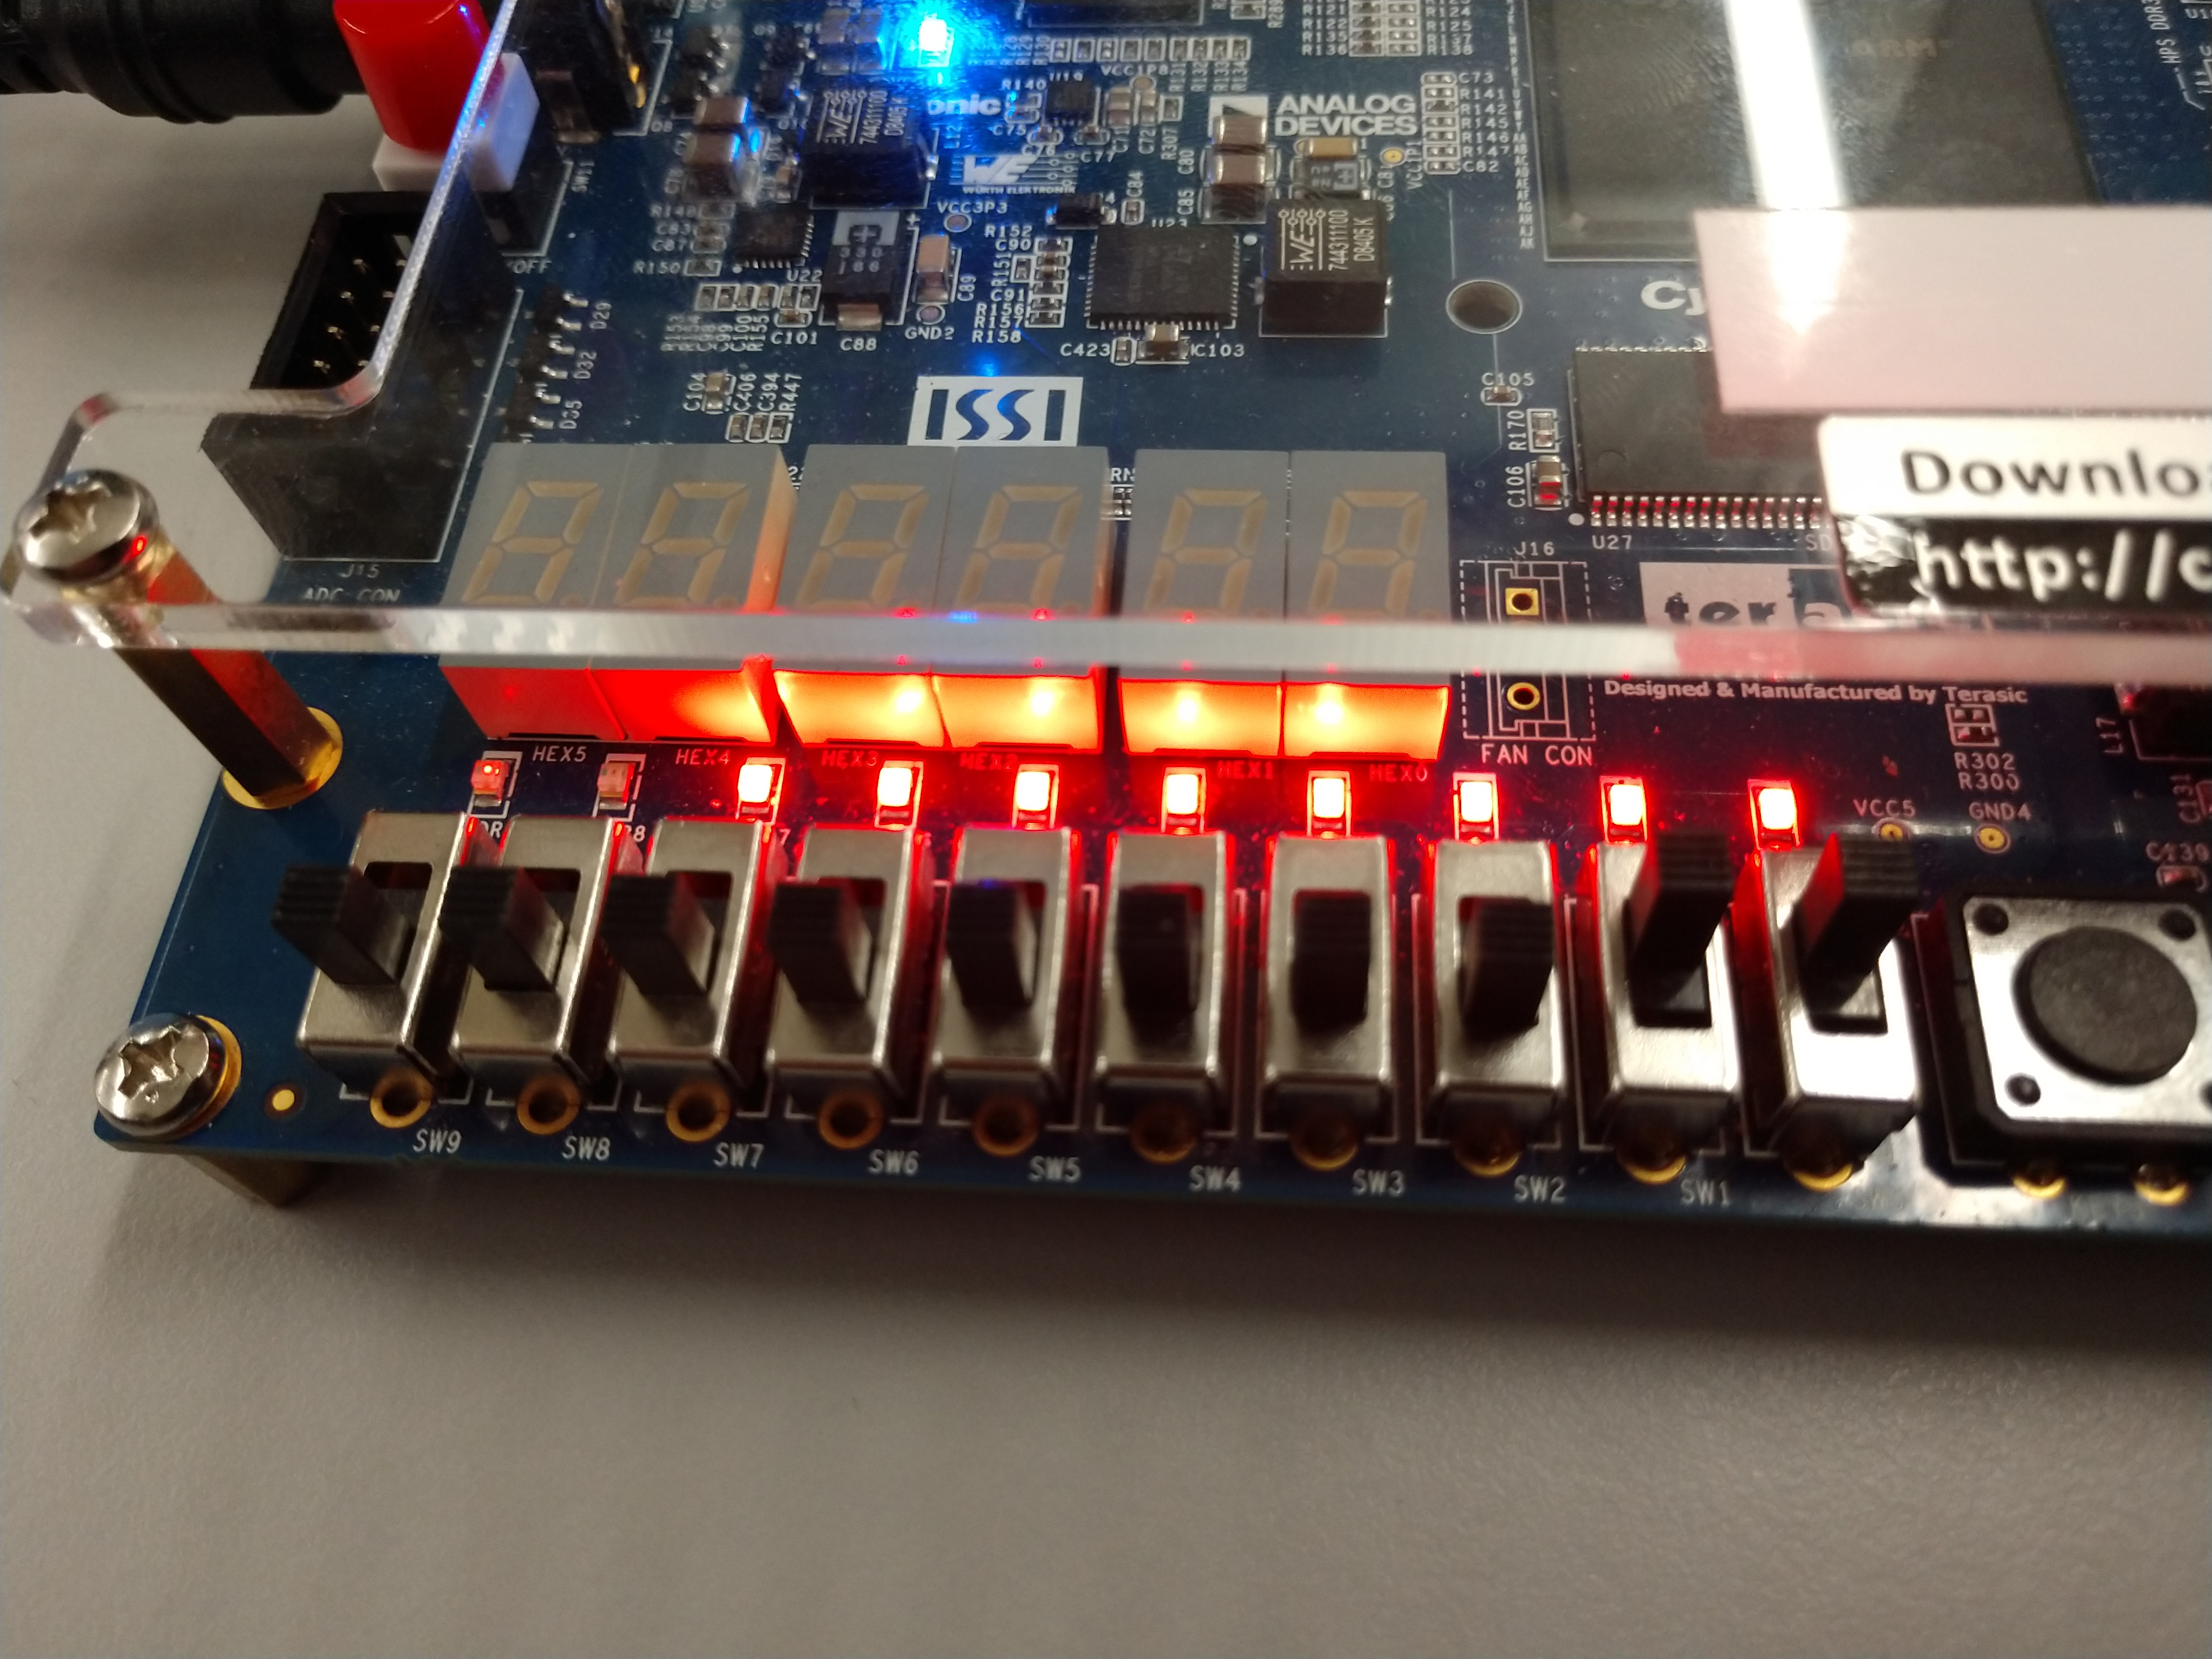
\includegraphics[width=.9\textwidth]{Figures/8BNormal.jpg}
  \caption{8-Bit Adder in a Non-Overflowed State}
  \label{fig:13}
\end{figure}

\end{document}
